\documentclass[12pt,a4paper]{report}
% UTU Project Report LaTex Format
% https://github.com/shahparth123/utu-report-format

%MIT License

%Copyright (c) 2019 Parth Shah

%Permission is hereby granted, free of charge, to any person obtaining a copy of this software and associated documentation files (the "Software"), to deal in the Software without restriction, including without limitation the rights to use, copy, modify, merge, publish, distribute, sublicense, and/or sell copies of the Software, and to permit persons to whom the Software is furnished to do so, subject to the following conditions: The above copyright notice and this permission notice shall be included in all copies or substantial portions of the Software. THE SOFTWARE IS PROVIDED "AS IS", WITHOUT WARRANTY OF ANY KIND, EXPRESS OR IMPLIED, INCLUDING BUT NOT LIMITED TO THE WARRANTIES OF MERCHANTABILITY, FITNESS FOR A PARTICULAR PURPOSE AND NONINFRINGEMENT. IN NO EVENT SHALL THE AUTHORS OR COPYRIGHT HOLDERS BE LIABLE FOR ANY CLAIM, DAMAGES OR OTHER LIABILITY, WHETHER IN AN ACTION OF CONTRACT, TORT OR OTHERWISE, ARISING FROM, OUT OF OR IN CONNECTION WITH THE SOFTWARE OR THE USE OR OTHER DEALINGS IN THE SOFTWARE.

% Enter your details in following lines:
\newcommand{\studentNameone}{Student Full Name}
\newcommand{\studentNametwo}{Student Full Name}
\newcommand{\studentNamethree}{Student Full Name}
\newcommand{\studentNamefour}{Student Full Name}
\newcommand{\guideName}{Mr. Guide Name}
\newcommand{\headName}{Mr. Head Name}
\newcommand{\directorName}{Mr. Director Name}
\newcommand{\enrollmentNumberone}{20XX02100XX000X}
\newcommand{\enrollmentNumbertwo}{20XX02100XX000X}
\newcommand{\enrollmentNumberthree}{20XX02100XX000X}
\newcommand{\enrollmentNumberfour}{20XX02100XX000X}
\newcommand{\reportTitle}{Project Title Project Title Project Title Project Title}
%\newcommand{\instituteName}{Chhotubhai Gopalbhai Patel Institute of Technology}
%\newcommand{\instituteNameshort}{CGPIT}
\newcommand{\instituteName}{Diwaliba Polytechnic}
\newcommand{\instituteNameshort}{Diwaliba Polytechnic}
\newcommand{\degreeName}{Diploma}
\newcommand{\branchName}{Branch Name}
\newcommand{\departmentName}{Department of CE/IT }
\newcommand{\locationName}{Mahuva, Surat}
\newcommand{\universityName}{Uka Tarsadia University}
\newcommand{\academicYear}{December-2019}

%***************************************************
% DO NOT CHANGE BELOW THIS LINE
%***************************************************
\usepackage[pdftex]{graphicx}
%\DeclareGraphicsExtensions{.pdf,.jpeg,.png}
\usepackage{graphicx} %for including images
\usepackage{setspace} %for line spacing
\usepackage{tabularx} %for basic spacing in caption and table
\renewcommand{\baselinestretch}{1.5}

\usepackage[pages=some]{background} %to add watermark
\backgroundsetup{                      %to add watermark
contents={
\includegraphics{UTU.png}},
angle=0,
scale=4,
color=black,
opacity=0.2
}

\usepackage{tocloft}    % tocloft for table of contents style

\usepackage[compact]{titlesec}  % titlesec for title section layout
\newcommand*{\justifyheading}{\raggedleft} % for right justification of chapters

%remove space before chapter title
\titleformat{\chapter}[display]
{\normalfont\huge\bfseries\justifyheading}{\chaptertitlename\ \thechapter}{20pt}{\Huge}
\titlespacing*{\chapter}{0pt}{-50pt}{40pt}


\renewcommand{\contentsname}{
\begin{center}
\LARGE\bf TABLE OF CONTENTS
\end{center}
} %for changing the contents title

\renewcommand\listtablename{
\begin{center}
\LARGE\bf LIST OF TABLES
\end{center}
} %for changing list of table title

\renewcommand\listfigurename{
\begin{center}
\LARGE\bf LIST OF FIGURES
\setlength\cftbeforefigskip{\cftbeforechapskip}
\end{center}
} %for changing list of figure title

\usepackage{subfig}

\renewcommand\cftchapafterpnum{\vskip6pt}   %for spacing change in table of content
\renewcommand\cftsecafterpnum{\vskip10pt}   %for spacing change in table of content
\renewcommand\cftsubsecafterpnum{\vskip10pt}
\renewcommand\cftsubsubsecafterpnum{\vskip10pt}

%--------------parth------------
\usepackage{color}   %May be necessary if you want to color links
\usepackage{hyperref}
\hypersetup{
    linktoc=all,     %set to all if you want both sections and subsections linked
    linkcolor=black  %choose some color if you want links to stand out
}
\usepackage{url}
\usepackage{notoccite}
\usepackage{float}
\usepackage{pdflscape}

%\usepackage{indentfirst }
%\usepackage{subcaption}
%%%%% For Removing paragraph
\setlength\parindent{0pt}
\setlength{\emergencystretch}{3em}

\usepackage{enumerate}
\newenvironment{tight_enumerate}{
 \begin{enumerate}
 \setlength{\topsep}{0pt}
 \setlength{\itemsep}{0pt}
 \setlength{\parskip}{0pt} }
{\end{enumerate}
}

\newenvironment{tight_itemize}{
 \begin{itemize}
 \setlength{\topsep}{0pt}
 \setlength{\itemsep}{0pt}
 \setlength{\parskip}{0pt} }
{\end{itemize}
}


\newenvironment{tight_description}{
 \begin{description}
 \setlength{\topsep}{0pt}
 \setlength{\itemsep}{0pt}
 \setlength{\parskip}{0pt} }
{\end{description}
}

%-----------------parth end----------------
%------------------------- Document settings ------------------------
\topmargin   0mm
\hoffset     0mm
\voffset     0mm
\textwidth   155mm
\textheight  230mm
%------------------------- Definitions ------------------------------



%------------------------- document ---------------------------------

\begin{document}
% --------- Title and abstract etc the front matter -----------
\pagenumbering{roman}
% TITLE PAGE

\thispagestyle{empty}

\begin{center}

{\large {A project report on}}
\vspace{0.6cm}

{\Huge \textbf{\reportTitle}}
\vspace{0.4cm}

{\large\textbf{by}}\\
{\large \bf \studentNameone} 
{\bf (\enrollmentNumberone)}\\
{\large \bf \studentNametwo} 
{\bf (\enrollmentNumbertwo)}\\
{\large \bf \studentNamethree} 
{\bf (\enrollmentNumberthree)}\\
{\large \bf \studentNamefour} 
{\bf (\enrollmentNumberfour)}\\
\vspace{0.9cm}

in partial fulfillment of the requirements for the degree of
\vspace{0.6cm}


{\large\textbf{\degreeName}}\\
{\large{in}}\\
{\large\textbf{\branchName}}\\
\vspace{0.5cm}
{\large{at}}\\
{\Large \textbf{\universityName}}
\vspace{0.6cm}

{\large\textbf{Under the guidance of}}\\
{\large \bf \guideName}
\vspace{0.1cm}

\begin{figure}[h]
\begin{center}
 
\includegraphics[scale=0.8]{UTU.png}
\end{center}
\end{figure}
{\bf \departmentName}\\
{\bf \instituteName}\\
{\bf \locationName}\\
{\bf \academicYear}
\end{center}

% -------------------------------------------------------------------------
\newpage
\addcontentsline{toc}{chapter}{CERTIFICATE}
\BgThispage

\begin{center}
{\LARGE \bf CERTIFICATE}\\
\end{center}
\vspace{0.8cm}
%\fontsize{12pt}{20pt}\selectfont
This is to certify that the project report entitled ``\textbf{\reportTitle}" has been carried out by \textbf{\studentNameone\ (\enrollmentNumberone)}, \  \textbf{\studentNametwo\ (\enrollmentNumbertwo)},\ \textbf{\studentNamethree \ (\enrollmentNumberthree)},\ \textbf{\studentNamefour\ (\enrollmentNumberfour)} at \textbf{\instituteName} for the partial fulfillment of \textbf{\degreeName}\ in\ \textbf{\branchName} \ degree to be awarded by \textbf{\universityName}.
\\
\\
\textbf{Date:}\\
\textbf{Place:} \locationName\\
\\
\\
\\
\\
\\
\\
\\
\begin{center}
\begin{tabular}{l l l}
\noindent \guideName  & \headName & \directorName \\
Guide, & Head, & Director,\\
\departmentName,& \departmentName, & \instituteNameshort \\
\instituteNameshort& \instituteNameshort & \universityName\\
\end{tabular}
\end{center}
\vspace{2cm} 
 
\begin{center}
  Examiner's Signature
\end{center}
% -------------------------------------------------------------------------
\newpage
\addcontentsline{toc}{chapter}{ACKNOWLEDGEMENT}
\begin{center}
{\LARGE \bf ACKNOWLEDGEMENT}\\
\end{center}
\vspace{0.8cm}

I have taken efforts in this seminar work. However, it would not have been possible
without the kind support and help of many individuals. I would like to extend my sincere thanks to all of them.

I am highly indebted to \textbf{\guideName} for his guidance and constant supervision as well as for providing necessary information regarding the seminar work.

I would like to express my gratitude towards my parents and member of family for their kind co-operation and encouragement which help me in completion of this project.
My thanks and appreciations also go to people who have willingly helped me out with
their abilities.


\begin{flushright}
\textbf{\studentNameone}\\
\textbf{\studentNametwo}\\
\textbf{\studentNamethree}\\
\textbf{\studentNamefour}
\end{flushright}


%---------------------------------------------------------------------------
\newpage
\addcontentsline{toc}{chapter}{ABSTRACT}
\begin{center}
{\LARGE \bf ABSTRACT}\\
\end{center}
\vspace{0.8cm}

\emph{Virtualization is a method of running multiple independent virtual operating systems
on a single physical computer. All the guest operating systems are completely isolated
It is a way of maximizing utilization of physical resources in order to minimize
investment in hardware. It also increase total productivity of the hardware. It has
been around since the first mainframe systems. This seminar mainly focuses on
virtualization as it pertains in any organization, but before considering any type of
server virtualization, it's important to define what technology or category of service
you're trying to virtualizes. Generally speaking, virtualization falls into three
categories: Operating System, Network, and Applications. All these categories
depends on one other. We can achieve scalability , reduce cost and reduce risk of
failure.}

%---------------------------------------------------------------------------


\begin{singlespace}

\newpage
\setlength{\cftbeforetoctitleskip}{-4em}  %for removing space before table of content title
\tableofcontents
\newpage
\addcontentsline{toc}{chapter}{LIST OF TABLES}
\setlength{\cftbeforelottitleskip}{-4em}  %for removing space before list of tables title
\listoftables
\newpage
\addcontentsline{toc}{chapter}{LIST OF FIGURES}
\setlength{\cftbeforeloftitleskip}{-4em}   %for removing space before list of figures title
\listoffigures
\end{singlespace}

\newpage
\addcontentsline{toc}{chapter}{LIST OF ABBREVIATIONS}\index{Abbreviations}
%\listofabbrevations
\begin{center}
{\LARGE \bf LIST OF ABBREVIATIONS}\\
\end{center}
\vspace{1.6cm}
AI \dotfill Artificial Intelligence\\
ANN \dotfill Artificial Neural Networks\\
BLEU \dotfill Bilingual Evaluation Understudy\\
CNN \dotfill Convolutional Neural Networks\\
%DIGITS \dotfill Deep Learning GPU Training System\\
GPU \dotfill Graphics Processing Unit\\
%ILVRC \dotfill ImageNet Large Scale Visual Recognization Challange\\
LSTM \dotfill Long Short Term Memory\\
MNIST \dotfill Mixed National Institute of Standards and Technology\\
NIST \dotfill National Institute of Standards and Technology\\
NN \dotfill Neural Network\\
NMT \dotfill Neural Machine Translation\\
RNN \dotfill Recurrent Neural Network\\


\newpage
\pagenumbering{arabic}
\pagestyle{headings}
% ----------------- thesis chapters -----------
% ----Introduction----------
\flushbottom
\chapter{Introduction}\label{Introduction}
Lorem ipsum dolor sit, amet consectetur adipisicing elit. Eos repudiandae dolor illum adipisci quod minus sequi impedit. Error delectus dolores, tempore suscipit at, nulla, voluptatem eum obcaecati perspiciatis modi eos\\

Lorem ipsum dolor sit, amet consectetur adipisicing elit. Eos repudiandae dolor illum adipisci quod minus sequi impedit. Error delectus dolores, tempore suscipit at, nulla, voluptatem eum obcaecati perspiciatis modi eos. Lorem ipsum dolor sit, amet consectetur adipisicing elit. Eos repudiandae dolor illum adipisci quod minus sequi impedit. Error delectus dolores, tempore suscipit at, nulla, voluptatem eum obcaecati perspiciatis modi eos.

\section{Overview}
 Lorem ipsum dolor sit, amet consectetur adipisicing elit. Eos repudiandae dolor illum adipisci quod minus sequi impedit. Error delectus dolores, tempore suscipit at, nulla, voluptatem eum obcaecati perspiciatis modi eos.Lorem ipsum dolor sit, amet consectetur adipisicing elit. Eos repudiandae dolor illum adipisci quod minus sequi impedit. Error delectus dolores, tempore suscipit at, nulla, voluptatem eum obcaecati perspiciatis modi eos.\\

Lorem ipsum dolor sit, amet consectetur adipisicing elit. Eos repudiandae dolor illum adipisci quod minus sequi impedit. Error delectus dolores, tempore suscipit at, nulla, voluptatem eum obcaecati perspiciatis modi eos.Lorem ipsum dolor sit, amet consectetur adipisicing elit. Eos repudiandae dolor illum adipisci quod minus sequi impedit. Error delectus dolores, tempore suscipit at, nulla, voluptatem eum obcaecati perspiciatis modi eos.\\

Lorem ipsum dolor sit, amet consectetur adipisicing elit. Eos repudiandae dolor illum adipisci quod minus sequi impedit. Error delectus dolores, tempore suscipit at, nulla, voluptatem eum obcaecati perspiciatis modi eos.Lorem ipsum dolor sit, amet consectetur adipisicing elit. Eos repudiandae dolor illum adipisci quod minus sequi impedit. Error delectus dolores, tempore suscipit at, nulla, voluptatem eum obcaecati perspiciatis modi eos.

\begin{figure}[h]
  \centering
  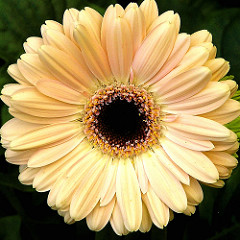
\includegraphics[width=13cm]{img/daisy}
  \caption{Some image name}\label{MLNNDL}
\end{figure}

 Lorem ipsum dolor sit, amet consectetur adipisicing elit. Eos repudiandae dolor illum adipisci quod minus sequi impedit. Error delectus dolores, tempore suscipit at, nulla, voluptatem eum obcaecati perspiciatis modi eos.Lorem ipsum dolor sit, amet consectetur adipisicing elit. Eos repudiandae dolor illum adipisci quod minus sequi impedit. Error delectus dolores, tempore suscipit at, nulla, voluptatem eum obcaecati perspiciatis modi eos.Lorem ipsum dolor sit, amet consectetur adipisicing elit. Eos repudiandae dolor illum adipisci quod minus sequi impedit. Error delectus dolores, tempore suscipit at, nulla, voluptatem eum obcaecati perspiciatis modi eos.Lorem ipsum dolor sit, amet consectetur adipisicing elit. Eos repudiandae dolor illum adipisci quod minus sequi impedit. Error delectus dolores, tempore suscipit at, nulla, voluptatem eum obcaecati perspiciatis modi eos.\\

As we can see in Figure \ref{learningsteps} process of learning can be divided in two parts:
\begin{tight_enumerate}
  \item Training
  \item Inference
\end{tight_enumerate}

  \begin{figure}[H]
  \centering
  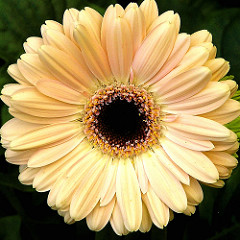
\includegraphics[width=10cm]{img/daisy}
  \caption[Image Name]{Image Name}\label{learningsteps}
\end{figure}

\section{Problem definition}

Lorem ipsum dolor sit, amet consectetur adipisicing elit. Eos repudiandae dolor illum adipisci quod minus sequi impedit. Error delectus dolores, tempore suscipit at, nulla, voluptatem eum obcaecati perspiciatis modi eos.Lorem ipsum dolor sit, amet consectetur adipisicing elit. Eos repudiandae dolor illum adipisci quod minus sequi impedit. Error delectus dolores, tempore suscipit at, nulla, voluptatem eum obcaecati perspiciatis modi eos.Lorem ipsum dolor sit, amet consectetur adipisicing elit. Eos repudiandae dolor illum adipisci quod minus sequi impedit. Error delectus dolores, tempore suscipit at, nulla, voluptatem eum obcaecati perspiciatis modi eos.Lorem ipsum dolor sit, amet consectetur adipisicing elit. Eos repudiandae dolor illum adipisci quod minus sequi impedit. Error delectus dolores, tempore suscipit at, nulla, voluptatem eum obcaecati perspiciatis modi eos. This was only possible due to 3 main things:

\begin{itemize}
  \item Lorem ipsum dolor sit, amet consectetur adipisicing elit. 
  \item Lorem ipsum dolor sit, amet consectetur adipisicing elit. 
  \item Lorem ipsum dolor sit, amet consectetur adipisicing elit. 
\end{itemize}

Lorem ipsum dolor sit, amet consectetur adipisicing elit. Eos repudiandae dolor illum adipisci quod minus sequi impedit. Error delectus dolores, tempore suscipit at, nulla, voluptatem eum obcaecati perspiciatis modi eos.Lorem ipsum dolor sit, amet consectetur adipisicing elit. Eos repudiandae dolor illum adipisci quod minus sequi impedit. Error delectus dolores, tempore suscipit at, nulla, voluptatem eum obcaecati perspiciatis modi eos.Lorem ipsum dolor sit, amet consectetur adipisicing elit. Eos repudiandae dolor illum adipisci quod minus sequi impedit. Error delectus dolores, tempore suscipit at, nulla, voluptatem eum obcaecati perspiciatis modi eos.Lorem ipsum dolor sit, amet consectetur adipisicing elit. Eos repudiandae dolor illum adipisci quod minus sequi impedit. Error delectus dolores, tempore suscipit at, nulla, voluptatem eum obcaecati perspiciatis modi eos.

\section{Scope}
Lorem ipsum dolor sit, amet consectetur adipisicing elit. Eos repudiandae dolor illum adipisci quod minus sequi impedit. Error delectus dolores, tempore suscipit at, nulla, voluptatem eum obcaecati perspiciatis modi eos.Lorem ipsum dolor sit, amet consectetur adipisicing elit. Eos repudiandae dolor illum adipisci quod minus sequi impedit. Error delectus dolores, tempore suscipit at, nulla, voluptatem eum obcaecati perspiciatis modi eos.

\flushbottom
%%-------------------------------------------------------------------------
% ----System Planning---------
\flushbottom
\chapter{System Planning}\label{System Planning}
\section{Project development approach}
Lorem ipsum dolor sit, amet consectetur adipisicing elit. Eos repudiandae dolor illum adipisci quod minus sequi impedit. Error delectus dolores, tempore suscipit at, nulla, voluptatem eum obcaecati perspiciatis modi eos.Lorem ipsum dolor sit, amet consectetur adipisicing elit. Eos repudiandae dolor illum adipisci quod minus sequi impedit. Error delectus dolores, tempore suscipit at, nulla, voluptatem eum obcaecati perspiciatis modi eos.
\section{System modules}
Lorem ipsum dolor sit, amet consectetur adipisicing elit. Eos repudiandae dolor illum adipisci quod minus sequi impedit. Error delectus dolores, tempore suscipit at, nulla, voluptatem eum obcaecati perspiciatis modi eos.Lorem ipsum dolor sit, amet consectetur adipisicing elit. Eos repudiandae dolor illum adipisci quod minus sequi impedit. Error delectus dolores, tempore suscipit at, nulla, voluptatem eum obcaecati perspiciatis modi eos.
\section{Functional requirements}

Lorem ipsum dolor sit, amet consectetur adipisicing elit. Eos repudiandae dolor illum adipisci quod minus sequi impedit. Error delectus dolores, tempore suscipit at, nulla, voluptatem eum obcaecati perspiciatis modi eos.Lorem ipsum dolor sit, amet consectetur adipisicing elit. Eos repudiandae dolor illum adipisci quod minus sequi impedit. Error delectus dolores, tempore suscipit at, nulla, voluptatem eum obcaecati perspiciatis modi eos. 

 Here is what a typical project looks like:

\begin{figure}[h]
\begin{center}
     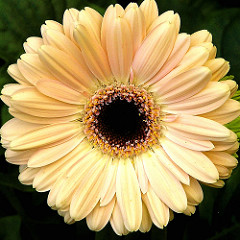
\includegraphics[width=13cm,height=5cm]{img/daisy}
     \caption[Architecture of project]{Architecture of project}
     \label{rnn}
\end{center}
\end{figure}
The Figure \ref{rnn} shows a RNN being unrolled (or unfolded) into a full network. Lorem ipsum dolor sit, amet consectetur adipisicing elit. Eos repudiandae dolor illum adipisci quod minus sequi impedit. Error delectus dolores, tempore suscipit at, nulla, voluptatem eum obcaecati perspiciatis modi eos.Lorem ipsum dolor sit, amet consectetur adipisicing elit.

Lorem ipsum dolor sit, amet consectetur adipisicing elit. Eos repudiandae dolor illum adipisci quod minus sequi impedit. Error delectus dolores, tempore suscipit at, nulla, voluptatem eum obcaecati perspiciatis modi eos.Lorem ipsum dolor sit, amet consectetur adipisicing elit. Eos repudiandae dolor illum adipisci quod minus sequi impedit. Error delectus dolores, tempore suscipit at, nulla, voluptatem eum obcaecati perspiciatis modi eos. 

\section{Nonfunctional requirements}

Lorem ipsum dolor sit, amet consectetur adipisicing elit. Eos repudiandae dolor illum adipisci quod minus sequi impedit. Error delectus dolores, tempore suscipit at, nulla, voluptatem eum obcaecati perspiciatis modi eos.Lorem ipsum dolor sit, amet consectetur adipisicing elit. Eos repudiandae dolor illum adipisci quod minus sequi impedit. Error delectus dolores, tempore suscipit at, nulla, voluptatem eum obcaecati perspiciatis modi eos.
\begin{table}[H]
\caption{Comparison of different models}
\label{imagecaptioncompare}
\begin{centering}
\begin{tabular}{|c|c|}
\hline
\textbf{Approch} & \textbf{Result}\tabularnewline
\hline
\hline
AAAAAA & 11\tabularnewline
\hline
BBBBBB  & 28\tabularnewline
\hline
\end{tabular}
\par\end{centering}

\end{table}

In Table \ref{imagecaptioncompare} Lorem ipsum dolor sit, amet consectetur adipisicing elit. Eos repudiandae dolor illum adipisci quod minus sequi impedit. Error delectus dolores, tempore suscipit at, nulla, voluptatem eum obcaecati perspiciatis modi eos.Lorem ipsum dolor sit, amet consectetur adipisicing elit. Eos repudiandae dolor illum adipisci quod minus sequi impedit. Error delectus dolores, tempore suscipit at, nulla, voluptatem eum obcaecati perspiciatis modi eos.
\section{Timeline chart}

Lorem ipsum dolor sit, amet consectetur adipisicing elit. Eos repudiandae dolor illum adipisci quod minus sequi impedit. Error delectus dolores, tempore suscipit at, nulla, voluptatem eum obcaecati perspiciatis modi eos.Lorem ipsum dolor sit, amet consectetur adipisicing elit. Eos repudiandae dolor illum adipisci quod minus sequi impedit. Error delectus dolores, tempore suscipit at, nulla, voluptatem eum obcaecati perspiciatis modi eos.
\flushbottom
%%-------------------------------------------------------------------------

%%-------------------------------------------------------------------------
% ----System Design---------
\flushbottom
\chapter{System Design}\label{System Design}
\section{Use case diagram}
Lorem ipsum dolor sit, amet consectetur adipisicing elit. Eos repudiandae dolor illum adipisci quod minus sequi impedit. Error delectus dolores, tempore suscipit at, nulla, voluptatem eum obcaecati perspiciatis modi eos.Lorem ipsum dolor sit, amet consectetur adipisicing elit. Eos repudiandae dolor illum adipisci quod minus sequi impedit. Error delectus dolores, tempore suscipit at, nulla, voluptatem eum obcaecati perspiciatis modi eos.
\section{Sequence diagram}
Lorem ipsum dolor sit, amet consectetur adipisicing elit. Eos repudiandae dolor illum adipisci quod minus sequi impedit. Error delectus dolores, tempore suscipit at, nulla, voluptatem eum obcaecati perspiciatis modi eos.Lorem ipsum dolor sit, amet consectetur adipisicing elit. Eos repudiandae dolor illum adipisci quod minus sequi impedit. Error delectus dolores, tempore suscipit at, nulla, voluptatem eum obcaecati perspiciatis modi eos.
\section{Activity diagram}
Lorem ipsum dolor sit, amet consectetur adipisicing elit. Eos repudiandae dolor illum adipisci quod minus sequi impedit. Error delectus dolores, tempore suscipit at, nulla, voluptatem eum obcaecati perspiciatis modi eos.Lorem ipsum dolor sit, amet consectetur adipisicing elit. Eos repudiandae dolor illum adipisci quod minus sequi impedit. Error delectus dolores, tempore suscipit at, nulla, voluptatem eum obcaecati perspiciatis modi eos.
\section{Class diagram}

Lorem ipsum dolor sit, amet consectetur adipisicing elit. Eos repudiandae dolor illum adipisci quod minus sequi impedit. Error delectus dolores, tempore suscipit at, nulla, voluptatem eum obcaecati perspiciatis modi eos.Lorem ipsum dolor sit, amet consectetur adipisicing elit. Eos repudiandae dolor illum adipisci quod minus sequi impedit. Error delectus dolores, tempore suscipit at, nulla, voluptatem eum obcaecati perspiciatis modi eos.
\section{E-R diagram}
Lorem ipsum dolor sit, amet consectetur adipisicing elit. Eos repudiandae dolor illum adipisci quod minus sequi impedit. Error delectus dolores, tempore suscipit at, nulla, voluptatem eum obcaecati perspiciatis modi eos.Lorem ipsum dolor sit, amet consectetur adipisicing elit. Eos repudiandae dolor illum adipisci quod minus sequi impedit. Error delectus dolores, tempore suscipit at, nulla, voluptatem eum obcaecati perspiciatis modi eos.

\section{Data flow diagram}
Lorem ipsum dolor sit, amet consectetur adipisicing elit. Eos repudiandae dolor illum adipisci quod minus sequi impedit. Error delectus dolores, tempore suscipit at, nulla, voluptatem eum obcaecati perspiciatis modi eos.Lorem ipsum dolor sit, amet consectetur adipisicing elit. Eos repudiandae dolor illum adipisci quod minus sequi impedit. Error delectus dolores, tempore suscipit at, nulla, voluptatem eum obcaecati perspiciatis modi eos.
\section{Database schema}
Lorem ipsum dolor sit, amet consectetur adipisicing elit. Eos repudiandae dolor illum adipisci quod minus sequi impedit. Error delectus dolores, tempore suscipit at, nulla, voluptatem eum obcaecati perspiciatis modi eos.Lorem ipsum dolor sit, amet consectetur adipisicing elit. Eos repudiandae dolor illum adipisci quod minus sequi impedit. Error delectus dolores, tempore suscipit at, nulla, voluptatem eum obcaecati perspiciatis modi eos.
Lorem ipsum dolor sit, amet consectetur adipisicing elit. Eos repudiandae dolor illum adipisci quod minus sequi impedit. Error delectus dolores, tempore suscipit at, nulla, voluptatem eum obcaecati perspiciatis modi eos.Lorem ipsum dolor sit, amet consectetur adipisicing elit. Eos repudiandae dolor illum adipisci quod minus sequi impedit. Error delectus dolores, tempore suscipit at, nulla, voluptatem eum obcaecati perspiciatis modi eos.
\flushbottom
%%-------------------------------------------------------------------------

%%-------------------------------------------------------------------------
% ----Implementation and Testing---------
\flushbottom
\chapter{Implementation and Testing}\label{Implementation and Testing}
\section{System development environment}

\subsection{Platforms}
Lorem ipsum dolor sit, amet consectetur adipisicing elit. Eos repudiandae dolor illum adipisci quod minus sequi impedit. Error delectus dolores, tempore suscipit at, nulla, voluptatem eum obcaecati perspiciatis modi eos.Lorem ipsum dolor sit, amet consectetur adipisicing elit. Eos repudiandae dolor illum adipisci quod minus sequi impedit. Error delectus dolores, tempore suscipit at, nulla, voluptatem eum obcaecati perspiciatis modi eos.

\section{Implementation/Design screenshots}

Lorem ipsum dolor sit, amet consectetur adipisicing elit. Eos repudiandae dolor illum adipisci quod minus sequi impedit. Error delectus dolores, tempore suscipit at, nulla, voluptatem eum obcaecati perspiciatis modi eos.Lorem ipsum dolor sit, amet consectetur adipisicing elit.
\section{Test cases}

Lorem ipsum dolor sit, amet consectetur adipisicing elit. Eos repudiandae dolor illum adipisci quod minus sequi impedit. Error delectus dolores, tempore suscipit at, nulla, voluptatem eum obcaecati perspiciatis modi eos.Lorem ipsum dolor sit, amet consectetur adipisicing elit. Eos repudiandae dolor illum adipisci quod minus sequi impedit. Error delectus dolores, tempore suscipit at, nulla, voluptatem eum obcaecati perspiciatis modi eos.

\flushbottom
%%-------------------------------------------------------------------------

%%-------------------------------------------------------------------------
% ----Conclusion and Future Work---------
\flushbottom
\chapter{Conclusion and Future Work}\label{Conclusion and Future Work}
\section{Conclusion}

Lorem ipsum dolor sit, amet consectetur adipisicing elit. Eos repudiandae dolor illum adipisci quod minus sequi impedit. Error delectus dolores, tempore suscipit at, nulla, voluptatem eum obcaecati perspiciatis modi eos.Lorem ipsum dolor sit, amet consectetur adipisicing elit. Eos repudiandae dolor illum adipisci quod minus sequi impedit. Error delectus dolores, tempore suscipit at, nulla, voluptatem eum obcaecati perspiciatis modi eos.
\section{Future work}

Lorem ipsum dolor sit, amet consectetur adipisicing elit. Eos repudiandae dolor illum adipisci quod minus sequi impedit. Error delectus dolores, tempore suscipit at, nulla, voluptatem eum obcaecati perspiciatis modi eos.Lorem ipsum dolor sit, amet consectetur adipisicing elit. Eos repudiandae dolor illum adipisci quod minus sequi impedit. Error delectus dolores, tempore suscipit at, nulla, voluptatem eum obcaecati perspiciatis modi eos.
\flushbottom

%------------ Appendix ----------------
\flushbottom
\appendix
%\include{AppendixA}
\flushbottom

%%-------------------------------------------------------------------------
%-----------------publication---------------------------------------
%\flushbottom
%\chapter{List of publication}\label{publication}
%\begin{enumerate}[1.]
%  \item {Purvi Tandel, Sharada Valiveti, K P Agrawal and K. Kotecha: \textbf{"Non-repudiation in Ad Hoc Networks"},The 2010 International Conference on Future Generation Communication and Networking- MANET 2010, on December 13-15, 2010 in International Convention Center Jeju , Jeju Island, Korea, Communications in Computer and Information Science, 2010, Volume 120, pp. 405-415, (2010).}
%  \item {Paper titled  \textbf{"Witness Selection to Achieve Non-repudiation in Ad-hoc Networks"} selected in the 2011 International Conference on Wireless and Optical Communications, may 21-22, Zhengzhou, China. The conference proceeding will be published by IEEE press in IEEE Xplore.}
%\end{enumerate}
\begin{enumerate}
  \item {Purvi Tandel, Sharada Valiveti, K P Agrawal and K. Kotecha: \textbf{"Non-repudiation in Ad Hoc Networks"},The 2010 International Conference on Future Generation Communication and Networking- MANET 2010, on December 13-15, 2010 in International Convention Center Jeju , Jeju Island, Korea, Communications in Computer and Information Science, 2010, Volume 120, pp. 405-415, (2010).}
\end{enumerate}

%\flushbottom

%------------------------------------------------------------------------
% ------------ Bibliography---------------
\renewcommand{\bibname}{References}
\begin{singlespace}
\bibliographystyle{ieeetr}
%\bibliography{reference}

\begin{thebibliography}{50}
	\addcontentsline{toc}{chapter}{REFERENCES}
\bibitem[1]{ref1}{Zhou, L., Haas, Z.J.:"Securing Ad Hoc Networks", IEEE Network 13 (1999) 24–30.}
\bibitem[2]{ref2}{Yu, S., Zhang, Y., Song, C., Chen, K.: "A security architecture for Mobile Ad Hoc Networks", Proceedings of Asia-Pasific Advanced Network(APAN), 2004.}
\end{thebibliography}
\end{singlespace}
\end{document} 